本章介绍一种从单张RGB-D图像中进行6D物体位姿估计的实例级物体位姿估计方法。当前实例级物体位姿估计中的领先方法\cite{Sundermeyer2023BOPC2}依赖基于渲染的精调流程,在实时性上有一定的瓶颈。基于渲染的精调流程需要渲染器渲染出当前估计所对应的图像,渲染过程需要耗费较多的资源。为了规避渲染耗时的局限性,本章提出了基于层次化表面编码和对应关系剪枝的HiPose架构,该方法通过层次化的二进制表面编码以粗到精的方式建立观测点到模型表面区域的对应关系。与之前的稠密对应方法不同,该方法不直接估计观测点对应的模型对应点,而是通过采用点到表面匹配来估计对应表面,并迭代性地收缩表面,直到其转变为对应点,同时逐渐去除离群点。在公共基准数据集 LM-O、YCB-V 和 T-LESS 上进行的大量实验显示,该方法在不依赖精调流程的方案中表现最优,甚至能与那些相对耗时的基于渲染的方法相抗衡。尤为重要的是,该方法计算效率极高,这使其能够在对精度要求苛刻的实时关键应用场景中发挥作用。代码链接见 \url{https://github.com/lyltc1/HiPose}。

\section{引言}
在缺乏纹理和严重遮挡的场景中,6D物体位姿估计仍具有挑战。近期的一些仅基于RGB的研究\cite{su2022zebrapose}在处理遮挡方面表现良好,但因单目图像存在深度不确定性而造成了精度下降。而一些基于RGB-D的方法\cite{wang2019densefusion,he2020pvn3d,he2021ffb6d,zhou2023deep}提出了新的特征融合网络,以更好地利用RGB和深度信息,但在公共基准如BOP挑战赛\cite{Sundermeyer2023BOPC2}上的表现仍落后。相较之下,目前大多数最先进的方法通常先利用RGB图像估计位姿,然后利用深度信息进行基于迭代优化的位姿精调流程\cite{Rusinkiewicz2001EfficientVO,lipson2022coupled}。与之不同的是,HiPose直接利用RGB-D图像进行位姿估计能够提供更精确、更可靠的物体位姿估计。

该方法深度融合几何与色彩信息,实现了精准的位姿估计,无需依赖耗时的后处理优化步骤。借助RGB-D传感器提供的多模态数据(包括观测点到相机的距离等几何信息),构建了更为鲁棒的视觉表征。受ZebraPose\cite{su2022zebrapose}框架的启发,设计了HiPose新型网络架构,通过预测深度图像与物体模型之间的密集对应关系完成位姿估计。不同于ZebraPose采用的编码策略,提出了一种基于迭代离群点消除的渐进式优化机制,通过由粗到精的多阶段处理流程逐步剔除异常对应点,如\autoref{fig:HiPose方法概览}所示。这种改进的编码处理方式不仅充分利用了编码的层次化特征,还显著提升了对应关系的精度和鲁棒性,能够实现实时高精度的位姿估计。

\begin{figure}[ht]
    \centering
    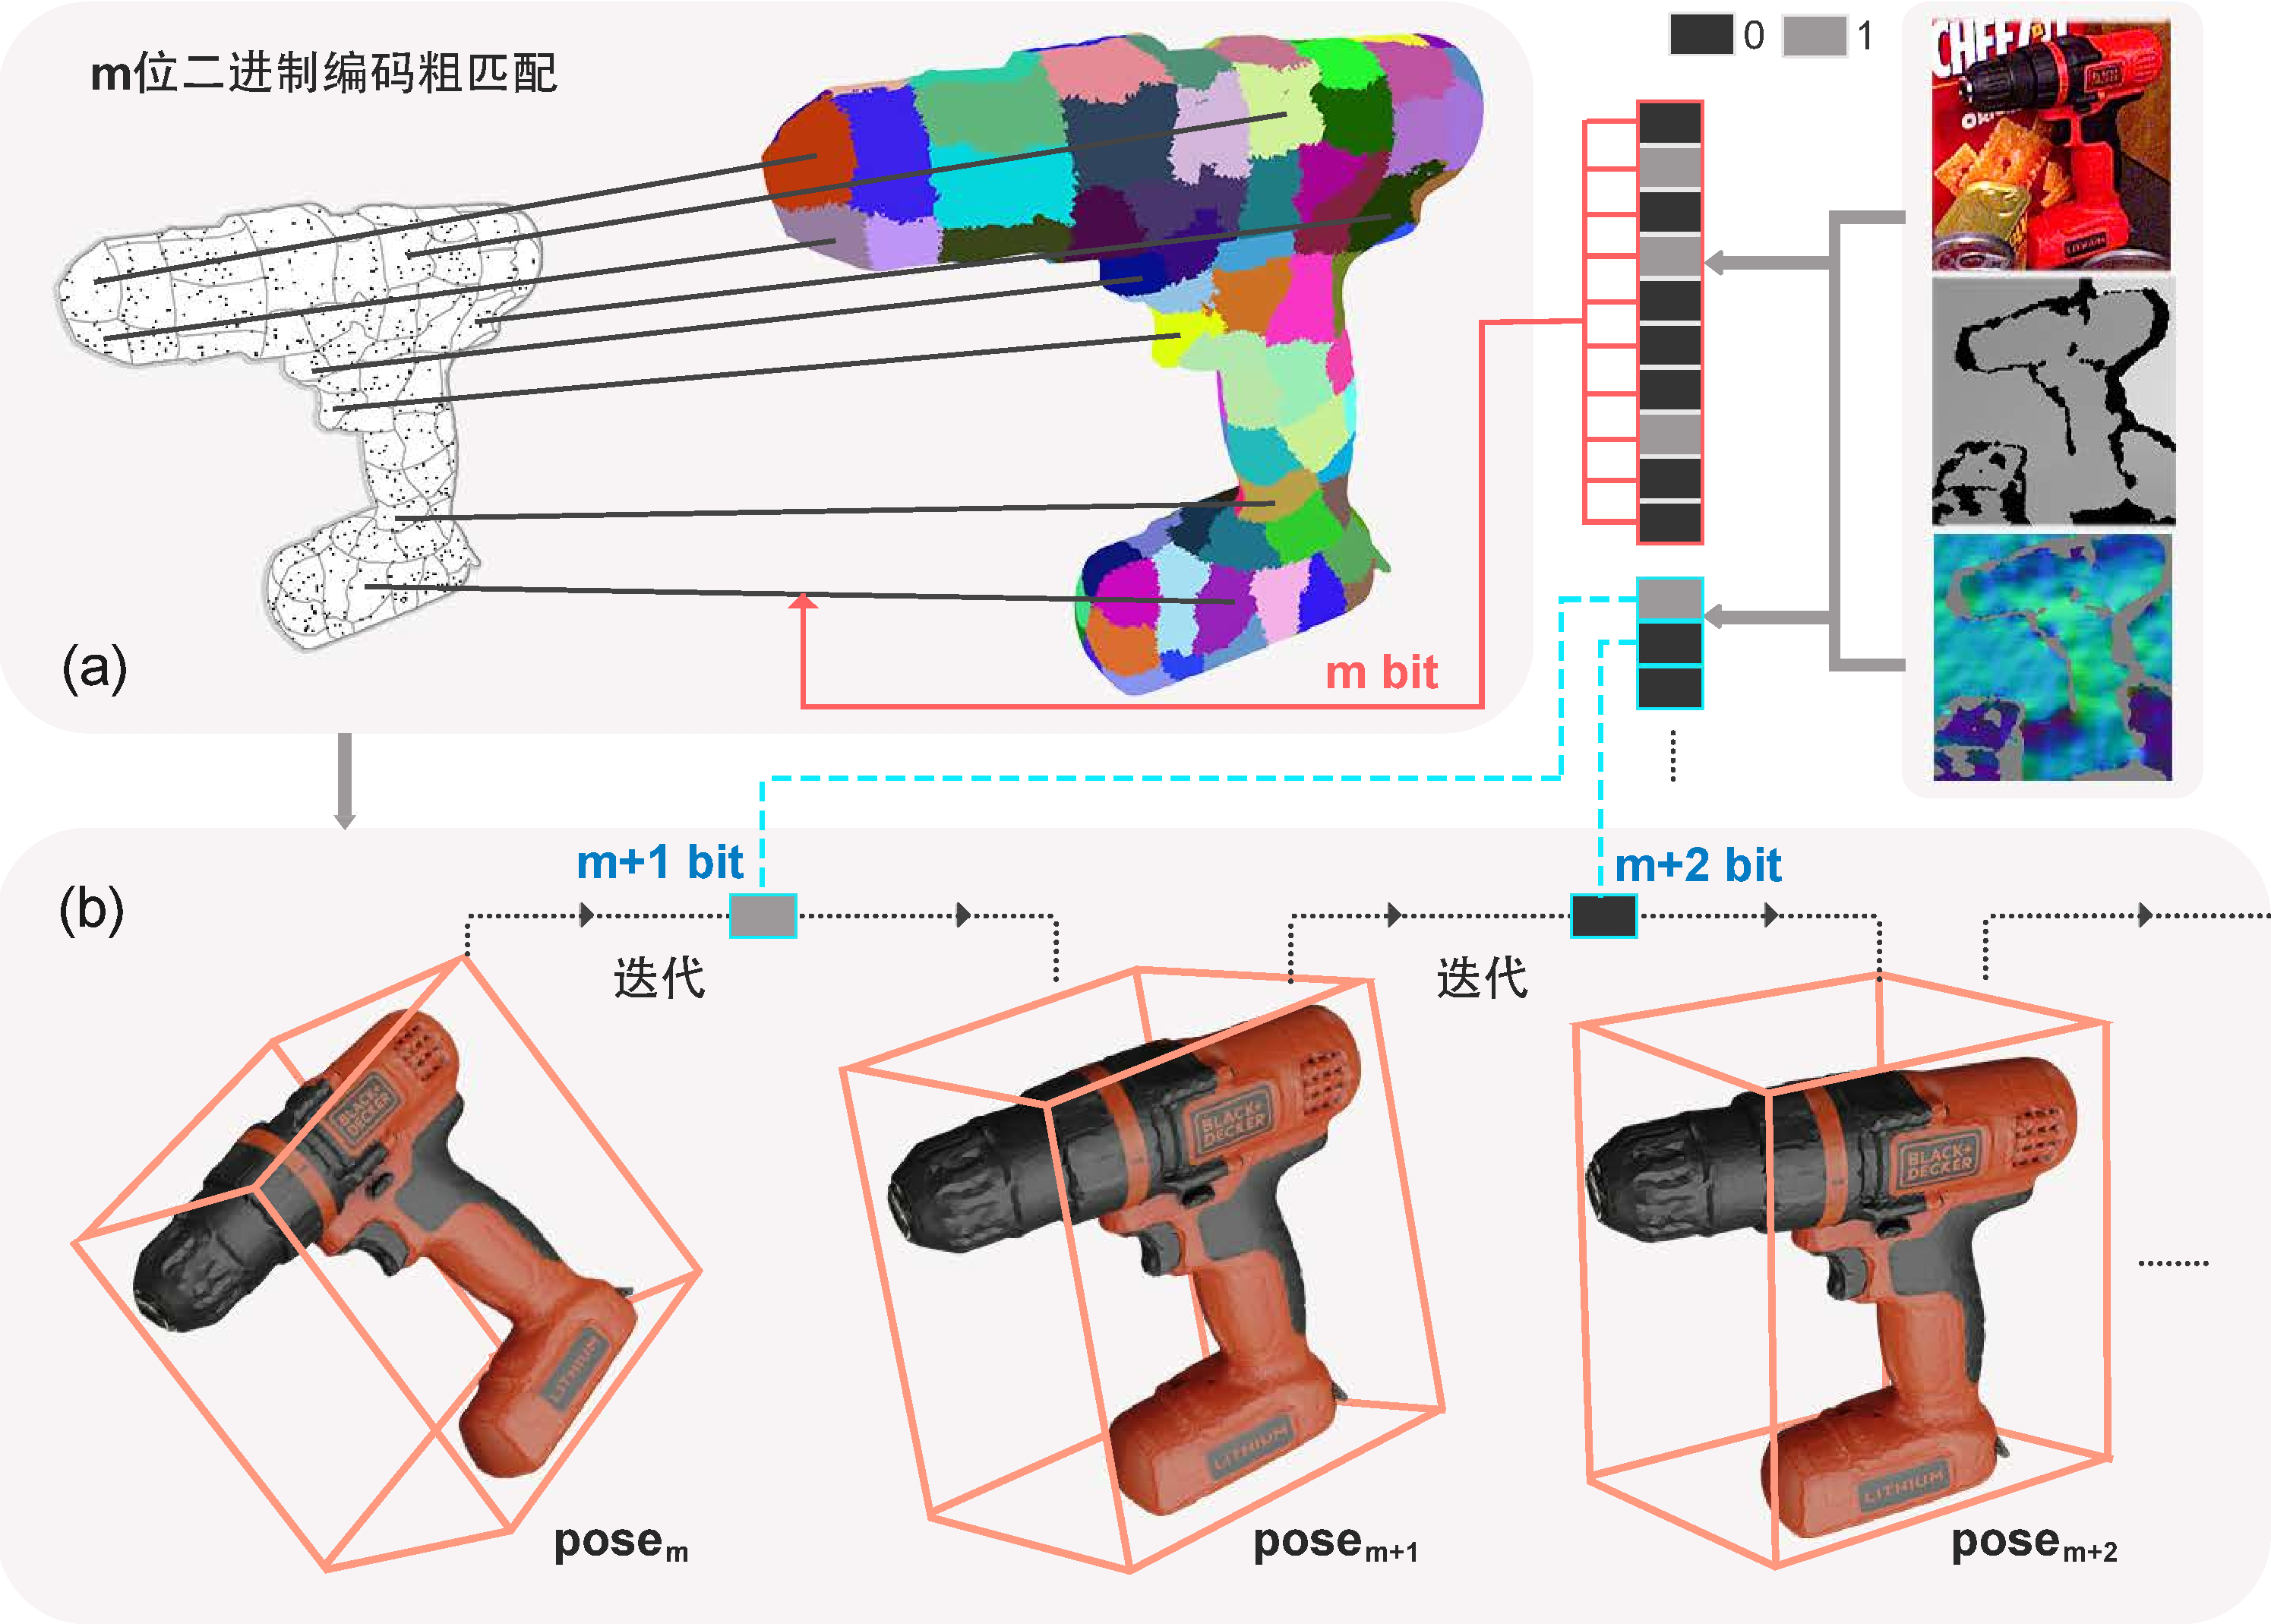
\includegraphics[width=0.75\linewidth]{hipose/teaser.pdf}
    \caption{HiPose的粗匹配和细匹配示意图}
    \label{fig:HiPose方法概览}
\end{figure}

本章提出了一种新颖且更稳定的层次化对应剪枝方法,摒弃了传统RANSAC框架下通过预测对应关系解决位姿问题的方式,例如常与Kabsch算法\cite{umeyama1991least}结合的方法。具体而言,层次化二进制编码输出的粗略预测具有更高的鲁棒性,能够提供稳健的初始位姿。这一初始位姿通过点到表面距离的方式有效识别并剔除离群匹配点。在此基础上,每次迭代进一步应用更精细的预测,逐步优化位姿估计,并在更细粒度的层面上去除离群点,从而显著提升精度。

总体而言,本章的贡献可以总结如下:
\begin{itemize}
\item 提出了一种充分利用RGB-D数据的物体位姿估计方法,专注于通过层次化二进制表面编码进行3D-3D对应匹配。
\item 引入了一种基于层次化对应剪枝的RANSAC-free位姿估计方法,通过粗到精的子表面去除离群点。
\item 在LM-O、YCB-V和T-LESS数据集上的大量实验验证了该方法的有效性。在无需额外精细化处理的情况下,该方法实现了最先进的性能,同时显著快于其他方法,适用于实时应用场景。
\end{itemize}
